% ==========================================
% Technical Report - Framework ( waltj3 )
% ==========================================
\chapter{CAVE Rendering Framework}

\section{Idea}

The main goal of this framework is to provide a simple tool library to render \gls{osg} applications with Equalizer. \gls{osg} developers do not need a lot of knowledge of Equalizer. The \gls{crf} offers simple methods to pass the \gls{osg} scene graph to Equalizer for basic \gls{osg} applications with static scene graphs. Furthermore, it provides additional tools to handle more complex \gls{osg} applications with user input and highly dynamic scenes.

Nevertheless, the final application is compatible with most Equalizer configurations and supports most \gls{osg} features. For further information about this, have a look at the section \nameref{sec:crfLimitations} or \nameref{chap:Testing}.

\section{Design}
\subsection{Design Techniques}
The \gls{crf} abstracts the more complex Equalizer framework. Similar, to many common frameworks, the \emph{Hollywood Principle}\footnote{\emph{The Hollywood Principle} is a well known paradigm in software engineering. \emph{Don't call us, we call you}, meaning the implemented functions are called by the framework than the developer.} plays a major role in the Equalizer framework and therefore also in our \gls{crf}. To provide an easy interface for simple \gls{osg} applications, we implemented the \texttt{crfStarter} class in a facade pattern\footnote{The facade pattern is a software engineering design pattern commonly used in \gls{oo} programming. The name is in analogy to an architectural facade. A facade is an object that provides a simplified interface to a larger body of code, such as a class library.} manor. This class provides easily understandable functions, which pass the \gls{osg} scene graph to the framework and run it with Equalizer.

\section{Namespaces}
\begin{description}
	\item[namespace \texttt{eq}] \hfill\\The low-level standard Equalizer namespace. When using the basic \gls{crf} features, one should not have to care about this namespace.
	\item[namespace \texttt{osg, osgViewer, osgGA, $\dots$}] \hfill\\Naturally, the \gls{crf} uses some of the \gls{osg} classes.
	\item[namespace \texttt{eqOsg}] \hfill\\The basic implementation for rendering \gls{osg} scene graphs with Equalizer. This namespace contains the implementations of all the must-have Equalizer classes to build a complete Equalizer application with a scene graph. Moreover, some basic features, like a camera control and the specialised \texttt{EqViewer}, which inherits from the standard \texttt{osgViewer}, are implemented here.
	\item[namespace \texttt{crf}] \hfill\\This namespace provides classes to abstract the \texttt{eqOSG} Equalizer application. Classes like \texttt{crfPipe}, \texttt{crfChannel} and the facade class \texttt{crfStarter} provide easily usable functions to run an \gls{osg} scene graph with Equalizer.
\end{description} 

\begin{figure}[H]
	\centering
		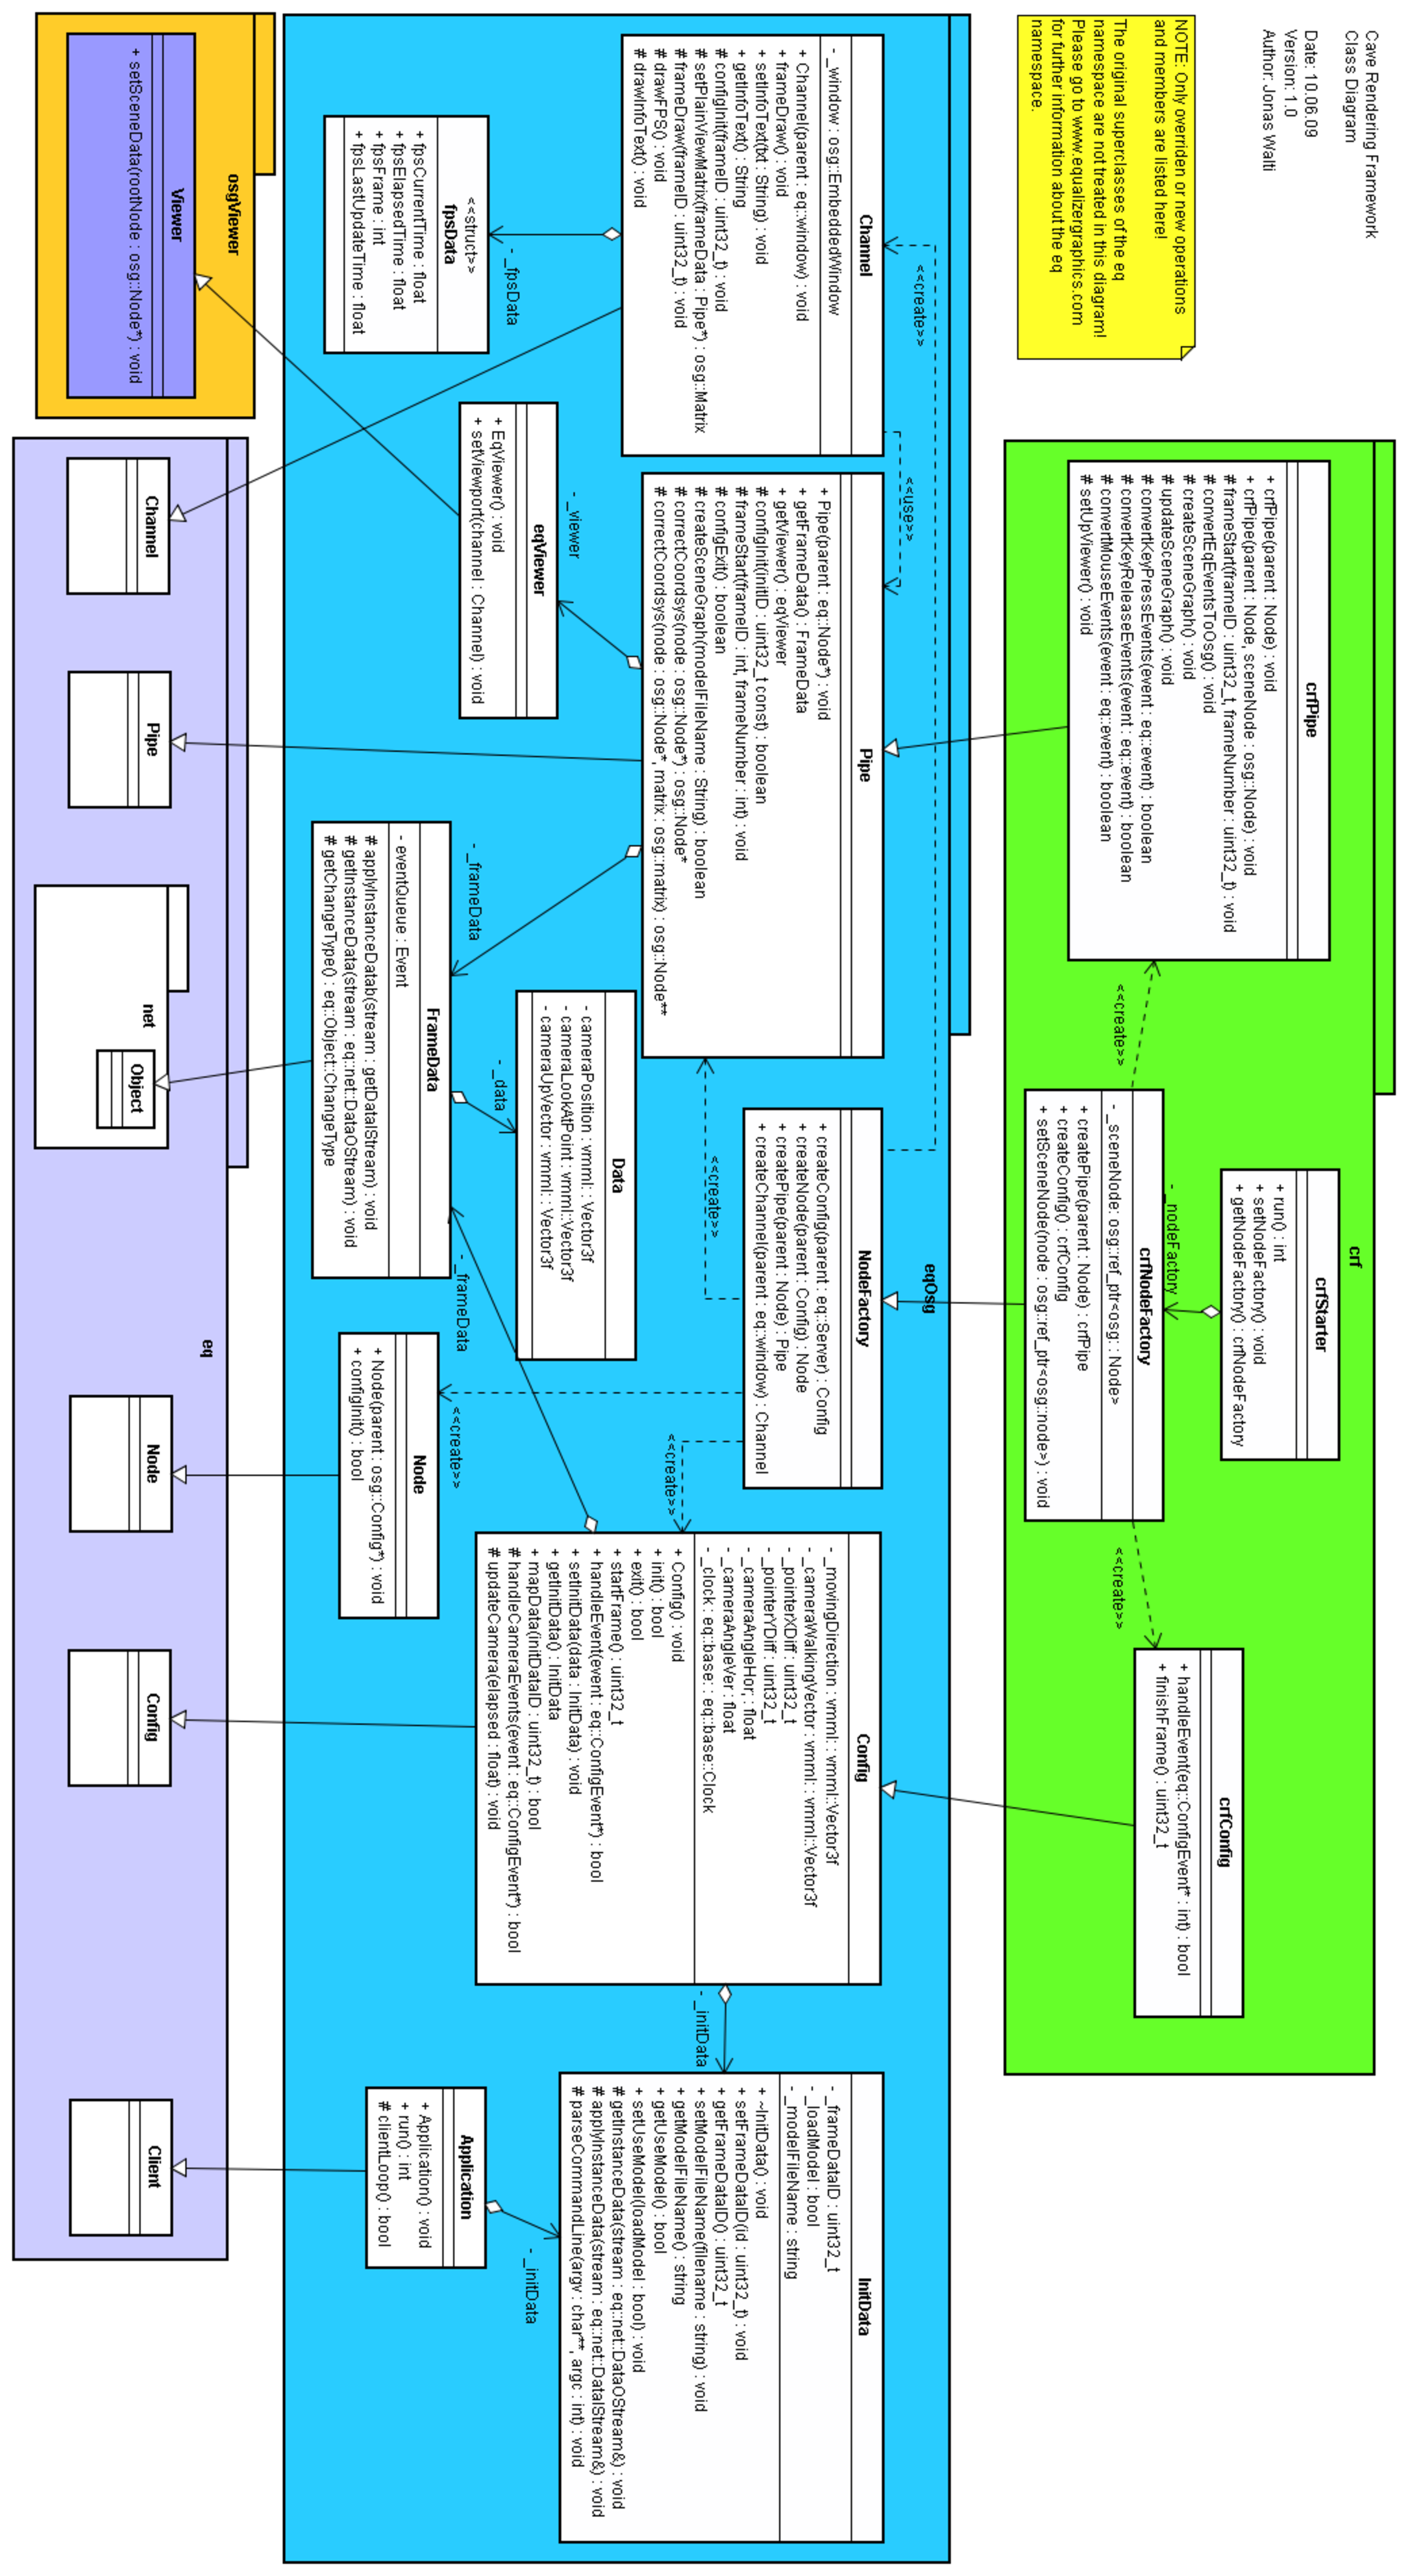
\includegraphics[width=0.850\textwidth,angle=180]{../figures/crf_class_diagram_complete_01}
	\caption{The complete class diagram with all three namespaces}
	\label{fig:crf_class_diagram_complete_01}
\end{figure}

\section{Implementation}
\subsection{About this section}
The information provided in this section cares about technical implementation facts. This may help a framework user to fix errors.

IMPORTANT: This part of the documentation requires knowledge of Equalizer. Please consult the previous Equalizer section or the Equalizer Programming Guide \cite{eqPG} for further information.

\subsection{Overview}
Equalizer applications in general are realised by subclassing existing classes of the \texttt{eq} namespace. A good example is the \texttt{eqPly} application, shipped with Equalizer. This example makes use of much Equalizer functionality. However, it has nothing to do with \gls{osg}.

In the \gls{crf} implementation, every pipe holds a complete \texttt{eqOsg::EqViewer}, which inherits from \texttt{osgViewer::Viewer}. Hence, every pipe holds a complete and fully independent scene graph. This is very important because this can force synchronisation problems and therefore errors in multipipe and/or multinode Equalizer configurations.

The only communication between this different scene graphs is realised with the \texttt{FrameData} class. \texttt{FrameData} inherits from the \texttt{eq::net::Object} class. This object has to be converted to a stream in order to pass it over the network in multinode configurations. In the basic \texttt{eqOsg::FrameData} class, several members are present to describe the cameras position, up-vector, viewing direction and current state. 

\subsection{\texttt{eqOsg} namepsace classes}
\label{sec:Overview}\hfill\\
Classes in the \texttt{eqOSG} namespace provide a basic Equalizer application with an \gls{osg} viewer. All needed functionality to render an \gls{osg} scene graph with Equalizer are implemented here.

\begin{description}
	\item [class \texttt{EqViewer}]\hfill\\
		The \texttt{EqViewer} class inherits from the original \texttt{osgViewer::viewer} and provides a viewer, which is used to render an \gls{osg} scene with Equalizer, because the default \texttt{osgViewer} does not work. Listing \ref{lst:eqViewer} shows the important line of code in the constructor.

	\begin{lstlisting}[caption={Constructor of the \texttt{EqViewer}},label={lst:eqViewer}]
	EqViewer::EqViewer()
	{
		//makes the viewer single threaded
		setThreadingModel(osgViewer::Viewer::SingleThreaded);

	}
	\end{lstlisting}
	Because a default \gls{osg} viewer does not support the multithreaded mode if configured as embedded window (what is needed here, because Equalizer creates the windows), the threading model is set to single. The newly added function \texttt{setViewport(eq::channel channel)} sets the frustum and the viewport of the camera, depending on the Equalizer configuration and the passed Equalizer channel.
	\item[class \texttt{Config}]\hfill\\
		As in a common Equalizer applications, \texttt{osgEq::Config} represents the current configuration of the application. It also updates the frame data class when necessary. Additionally, the \texttt{eqOsg::Config} class calculates the position and viewing direction of the camera. This happens by receiving mouse and keyboard events in \texttt{Config::handleEvents()}. Afterwards, calculating the new cameras properties in \texttt{Config::updateCamera()}. Finally, the new camera properties are updated in the frame data. \\ The rest is similar to the eqPly example.
	\item[class \texttt{FrameData}]\hfill\\
		The \texttt{FrameData} class is a container for values which can be sent to every node and pipe. This is the only way to pass (updated) data to the different render clients and pipes at runtime. In the \texttt{eqOsg::FrameData} class, all information concerning the camera is stored in this object.
	\item[class \texttt{Application}]\hfill\\
		The \texttt{eqOsg::Application} class is similar to the eqPly example. This class starts and stops the application, runs the main loop by calling the \texttt{startFrame()}, and \texttt{finishFrame()} functions of the \texttt{Config} object.
	\item[class \texttt{NodeFactory}]\hfill\\
		The \texttt{eqOsg::NodeFactory} is needed to create the desired objects during the initialisation of Equalizer.
	\item [class \texttt{Node}]\hfill\\
		As in a standard Equalizer application, the node class represents a render client. This class does not contain important changes, because the \gls{crf} does not need node-specific customisations.
	\item [class \texttt{Pipe}]\hfill\\
		The class \texttt{Pipe} abstracts a physical \gls{gpu}. The derived class \texttt{eqOsg::Pipe} holds the two additional members; The \texttt{osgEq::EqViewer} \texttt{\_viewer} and the \texttt{eqOsg::FrameData} \texttt{\_frameData}. The viewer holds the complete scene graph and frame data, which is a copy of the distributed data. \texttt{eqOsg::Pipe} is a basic and lightweight implementation with an empty scene graph. The \texttt{crf::crfPipe} inherits from this class and provides additional functions to create and update the scene graph. More information about this can be found in the following sections.% (\ref{sec:...}).
	\item [class \texttt{InitData}]\hfill\\
		The \texttt{eqOsg::InitData} class is needed during the initialisation of the application. It also provides a function to parse the command line and set this initial data. Furthermore, it holds the frame data ID, so all clients can synchronise on the distributed frame data object.
	\item [class \texttt{Channel}]\hfill\\
 		In Equalizer a \texttt{Channel} represents an \gls{opengl} viewport. Hence, \texttt{eqOsg::Channel} renders the scene graph. This is done with the \texttt{frameDraw()} function. Consult \ref{sec:FrameRendering} for more information. Moreover, when the \texttt{configInit} function of the channel is called, the \texttt{EqViewer} will be configured as an embedded window. This ensures that a virtual \gls{osg} window is defined, which is widely used in given \gls{osg} classes (for example \texttt{osgViewer::StatsHandler} or \texttt{osgGA::FlightManipulator}).
\end{description}

  
\subsection{\textbf{\texttt{crf}} namepsace classes}
\hfill\\
The \texttt{crf} namespace contains more specialised classes to render \gls{osg} applications with Equalizer. The lightweight  \texttt{eqOsg} namespace provides only basic features to render an \gls{osg} scene graph. The derived classes of the \texttt{crf} namespace implement additional functionality for showing statistics, scene graph coordinate system correction and the \texttt{crfStarter} class as a facade for simple execution of the application.
\begin{description}
	\item[class \texttt{crfNodeFactory}]\hfill\\
		This class inherits from the \texttt{eqOsg::NodeFactory} and is used by the \texttt{crfStarter} class to create the desired Equalizer objects.
	\item[class \texttt{crfStarter}]\hfill\\
		The \texttt{crfStarter} is the facade class of our framework. With this class it is possible to run an Equalizer \gls{osg} application with two lines of code shown in listing \ref{lst:crfStarter}.
		
		\begin{lstlisting}[caption={\texttt{crfStarter} main method},label={lst:crfStarter}]
		#include <crf/crfStarter.h>

		//1. Create the main method, which calls the crfStart.run() 
		//method to start equalizer and stuff
		int main(int argc, char** argv) 
		{
		    //create the \gls{crf} starter
			crf::crfStarter starter;

			//run the application
			starter.run(argc,argv);
		}
		\end{lstlisting}

		In this special case, a HelloWorld application will be started because no node factory and no \gls{osg} node have been passed to the starter object. For simple scene graphs, it is possible to pass an \gls{osg} root node as third argument of the \texttt{starter.run(...)} method. For dynamic and more complex \gls{osg} applications, custom classes have to be implemented (by subclassing the desired \texttt{eqOsg} and \texttt{crf} classes) and a custom node factory has to be passed to the starter with \texttt{starter.setNodeFactory(yourCustomFactory)}.
	\item[class \texttt{crfPipe}]\hfill\\
		This class extends the \texttt{eqOsg::Pipe} with features like pushing Equalizer events to the \gls{osg} viewer, scene graph updates, scene graph rotation and more. 
\end{description}

\subsection{OSG Rendering With Equalizer}
\subsubsection{Overview}
\label{sec:Overview}
This section explains how the scene graph is rendered with Equalizer. In the \emph{eqPly} or the \emph{eqHello} example of Equalizer, there is native OpenGL code in the \texttt{Channel::frameDraw()} function. But in the \gls{crf}, the OpenGL commands come from the \gls{osg} viewer's camera and have to be rendered considering every channel's viewing matrix. 

\subsubsection{Frame Rendering}
\label{sec:FrameRendering}
The \gls{osg} related rendering is done by the \texttt{eqOsg::Channel::frameDraw()} function. The code of \texttt{eqOsg::Channel::frameDraw()} is shown in listing \ref{lst:frameDraw}.

\begin{lstlisting}[caption={\texttt{Channel::frameDraw()}},label={lst:frameDraw}]
void Channel::frameDraw( const uint32_t frameID )
{
	// setup OpenGL State
	eq::Channel::frameDraw( frameID );
	
	// get the pipe and the viewer
	Pipe *pipe = static_cast<Pipe*>( getPipe() );
	osg::ref_ptr<EqViewer> viewer = pipe->getViewer();
	
	// set the correct viewport (which can change each frame)
	viewer->setViewport( this );
	
	// set a view matrix and make sure it is multiplied with the head
	// matrix of Equalizer
	osg::Matrix headView = setPlainViewMatrix( pipe );
	headView.postMult( vmmlToOsg( getHeadTransform() ) );
	//set the channels correct view matrix to the osgViewer's camera
	viewer->getCamera()->setViewMatrix( headView );
	
	// render the scene graph
  viewer->frame();
  
  ... more instructions for drawing statistic
}\end{lstlisting}

The important difference of the implementation of \texttt{Channel::frameDraw()} in the \emph{eqPly} example and in the \gls{crf} is that the drawing code is retrieved from the \texttt{osgViewer} of the pipe and is not directly realised with common \gls{opengl} commands. The frame of the viewer depends on the current main camera in the scene graph. Therefore, the correct properties (position, up-vector and viewing direction) for the camera need to be set to get the correct frame for each Equalizer channel. This very important step is done by the \texttt{eqOsg::Channel::frameDraw()} function, posted above. With \texttt{setPlaneViewMatrix(pipe)} the cameras position, up-vector and view direction is updated because the camera can be moved. This step is executed for every channel. 
After setting up the general camera properties, the cameras view matrix has to be defined. This is different for every channel and depends on the Equalizer configuration and the head matrix (which represents the viewers position and orientation). The \texttt{getHeadTransform()} function returns the correct view frustum and orientation for each channel defined in the Equalizer configuration. 
After multiplying the view matrix of the camera with the head transformation matrix of the channel, the result is set as the new view matrix for the camera of the channel.
Afterwards, the drawing code can be executed by calling \texttt{viewer->frame()}.

\paragraph{Summary}
\label{sec:Recap}
\begin{enumerate}
	\item call the base \texttt{frameDraw()} of the Equalizer base class to set-up the correct OpenGL state
	\item pass the viewport of the channel  to the \gls{osg} viewer
	\item get the current position, view direction and up-vector of the main camera of the scene graph
	\item multiply this with the head transformation matrix of the channel
	\item set the result as new view matrix for the camera of the channel
	\item render the frame
\end{enumerate}

\subsection{Event Handling}
\subsubsection{Equalizer Event Handling}
\label{sec:EqualizerEventhandling}\hfill\\
In the \texttt{eqOsg} and \texttt{crf} Equalizer implementation, the general event handling is done in the \texttt{Config} class. The \texttt{Config::handleEvents(ConfigEvent event)} function handles the Equalizer events. To get more information about the general event handling in Equalizer, consult the Equalizer Programming Guide \cite{eqPG}.

\subsubsection{CRF Event Handling}
\label{sec:crfEventHandling}
In \gls{osg} applications, it is very common to add multiple event handlers to the \texttt{osgViewer}. The \texttt{osgViewer} receives all the events directly, because in basic \gls{osg} applications this viewer creates its own window(s). In this project, Equalizer generates the windows and receives the events. To keep the possibility of using the common \gls{osg} event handlers, a mechanism is created that passes all the key and mouse related events from the \texttt{crf::crfConfig::handleEvents()} function via the \texttt{FrameData}'s \texttt{eventQueue} to every pipe. In the \texttt{crfPipe::frameStart()} function, Equalizer events are converted to \gls{osg} events and passed to the event queue of \texttt{eqOsg::EqViewer}. Everytime \texttt{crf::crfConfig::frameFinish()} is called, the eventQueue of \texttt{FrameData} is cleared because the events have already been pushed to the eventQueue of the \gls{osg} viewer by the pipe during the last \texttt{crfPipe::frameDraw()} call.

The three functions \texttt{convertKeyPressEvents(...)}, \texttt{convertKeyReleaseEvents(...)} and \texttt{convertMouseEvents(...)} convert the Equalizer events to \gls{osg} events and push them to the eventQueue of the viewer. Some basic conversions are done in the \texttt{crf::Pipe} class. To change these conversions and/or support additional keys, these functions have to be overridden. Unfortunately, this part of the \texttt{crf} depends on the operating system because each windowing system reports different ACSII codes. Moreover, Equalizer does not report all codes properly for some special keys. This is already tracked as a bug and should be fixed in future Equalizer releases.

\paragraph{Summary}
\begin{enumerate}
	\item \texttt{crf::crfConfig::handleEvent(event)} pushes the desired events (default: key and mouse events) to the \texttt{\_eventQueue} vector of the distributed \texttt{\_framedata} object
	\item \texttt{crf::crfConfig::handleEvent(event)} calls the eqOsg::Config::handleEvent(event) function
	\item depending on the handled events, the \texttt{\_framedata} object gets updated
	\item \texttt{eqOsg::Config::frameDraw()} commits the \texttt{\_framedata} object
	\item in \texttt{crf::crfPipe::frameStart} \texttt{convertKeyPressEvents}, \texttt{convertKeyReleaseEvents} and \texttt{convertKeyPressEvents} are called
	\item in these functions, the passed events are converted to \gls{osg} events and thereafter pushed to the event queue of the viewer (see figure \ref{fig:crf_seq_pipe_frame_draw_01})
\end{enumerate}

\begin{figure}[H]
	\centering
		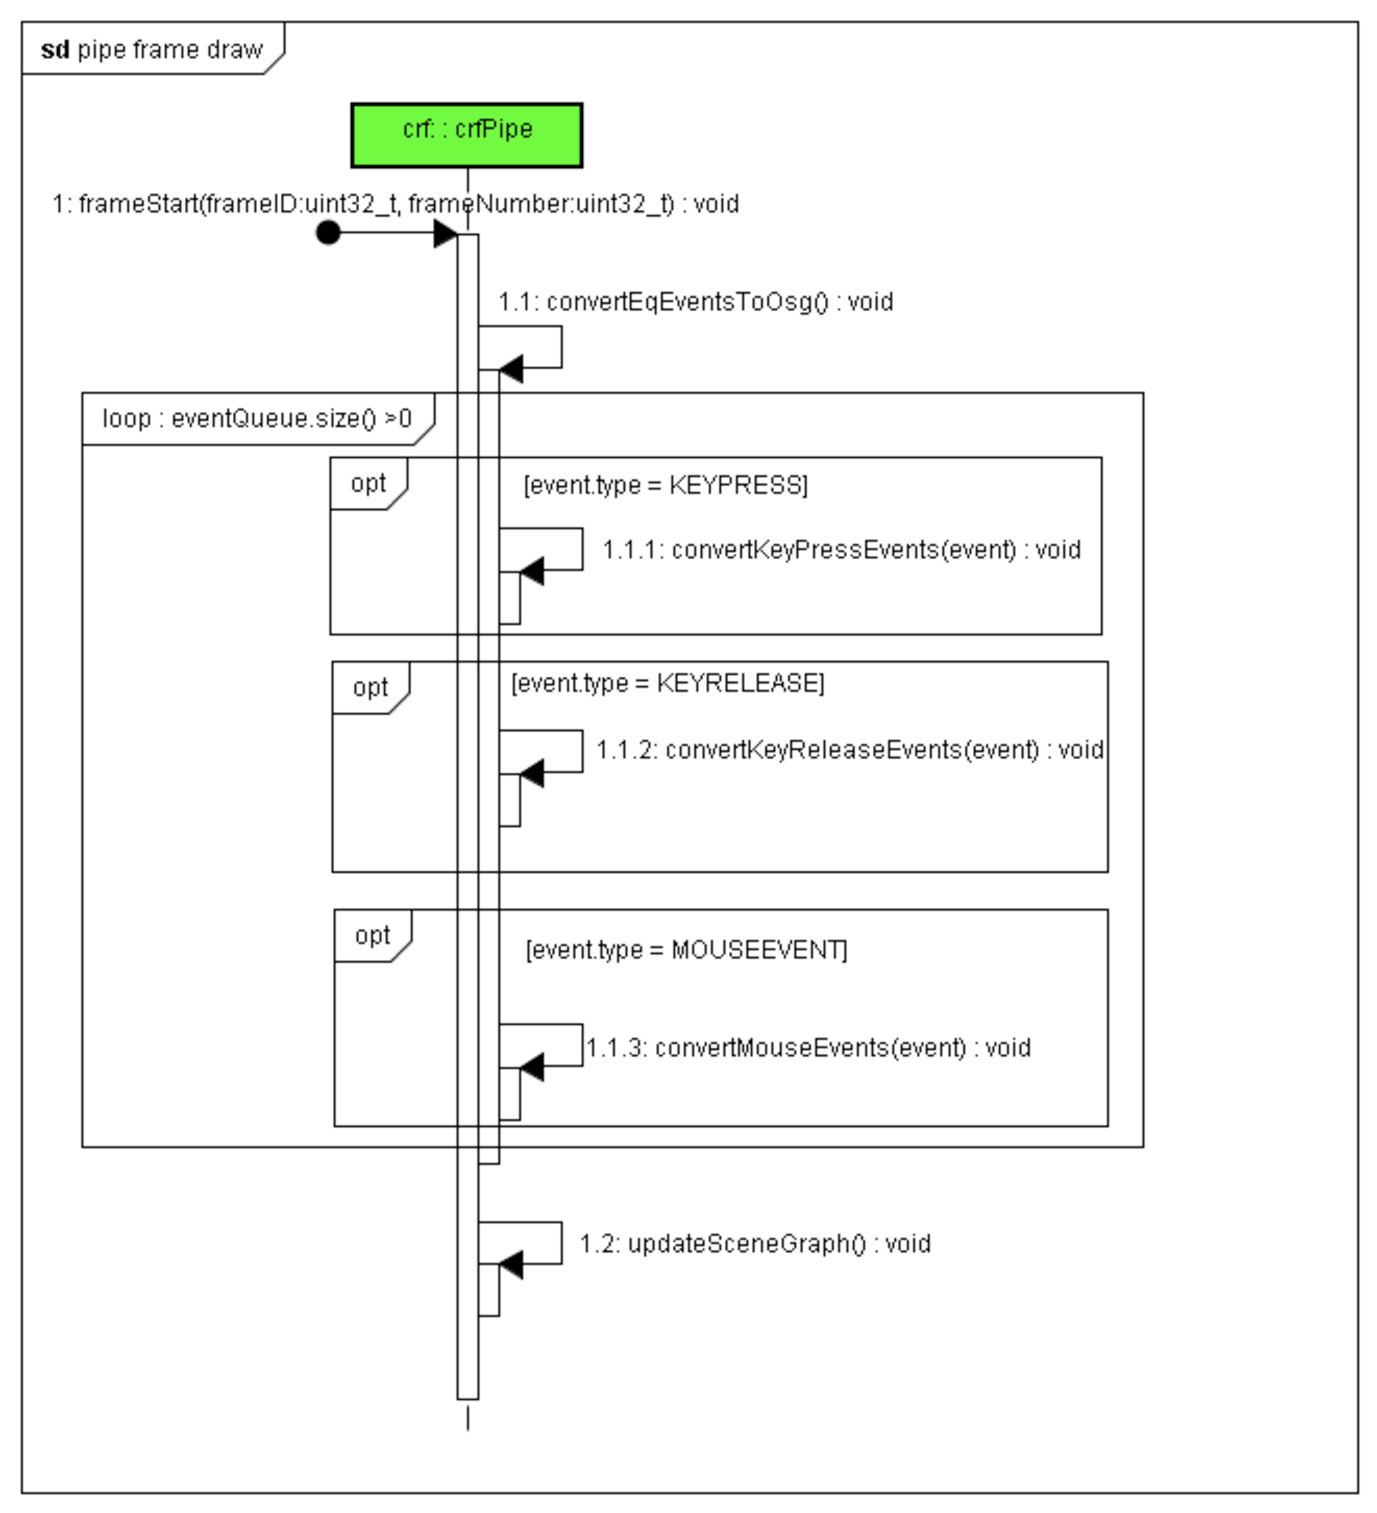
\includegraphics[width=0.70\textwidth]{../figures/crf_seq_pipe_frame_draw_01}
	\caption{the pipe's \texttt{frameDraw()} function as a sequence diagram }
	\label{fig:crf_seq_pipe_frame_draw_01}
\end{figure}

\section{Limitations}
\label{sec:crfLimitations}
\subsection{Scene Graph Creation}
Due to the fact that in Equalizer configurations with $n$ pipes on one node $n$ \gls{osg} scene graphs are created. The used objects in this creation-process must not be global and/or static. This is because every scene graph has to be completely independent and must not share the same memory. If static objects are used, every scene graph refers to the same memory on the node with several pipes. This causes errors or even segmentation faults.

\subsection{Dynamic Scene Graphs}
Changes in the scene graph have to be synchronised over all pipes and nodes. Due to the fact that distributed objects (the \texttt{FrameData} class at runtime and the \texttt{InitData} class on start-up in the \gls{crf}) provide the only way to communicate between pipes and nodes. 
%All scene graph changes have to be initiated due a distributed objects.
Common viewer bound \gls{osg} event handlers (like the \texttt{osgGA::TrackBallManipulator} or the \texttt{osgViewer::Statshandler}) can be used because the \gls{crf} sends all mouse and keyboard events to every viewer of every pipe with its \texttt{FrameData} class. 
To add other input devices like a 3D joystick or similar, the new events have to be pushed from the \texttt{Config} class over a distributed object to every pipe. Now, the scene graph's changes have to be made in the pipe. Due to the fact that the distributed objects are completely synchronised, every pipe receives the same events at the same time (frame). To summarise, all changes in a scene graph have to be caused by distributed data. In our case this responsibility is taken by the \texttt{FrameData} class.

\subsection{Model Loading with Multiple Pipes on One Machine}
Random segmentation faults occured when loading \gls{osg} models with \texttt{osgDB::loadNodeFile()} on a multipipe node with just one running instance of the CRF application. After some debugging efforts these random errors seem to be caused by a not thread-safe singleton pattern, used in \gls{osg}.
This error does not appear in multinode environments where on every node one instance of the \gls{crf} application runs per node and therefore the singleton pattern is processed properly.

\section{Previous Work}
This framework is based on the basic \gls{osg}-Equalizer application eqOSG, realised by a \gls{vr} research group of the University of Siegen. 